\documentclass[10pt,twocolumn,letterpaper]{article}

\usepackage{cvpr}
\usepackage{times}
\usepackage{epsfig}
\usepackage{graphicx}
\usepackage{amsmath}
\usepackage{amssymb}

% Include other packages here, before hyperref.

% If you comment hyperref and then uncomment it, you should delete
% egpaper.aux before re-running latex.  (Or just hit 'q' on the first latex
% run, let it finish, and you should be clear).
\usepackage[pagebackref=true,breaklinks=true,letterpaper=true,colorlinks,bookmarks=false]{hyperref}

\cvprfinalcopy % *** Uncomment this line for the final submission

\def\cvprPaperID{****} % *** Enter the CVPR Paper ID here
\def\httilde{\mbox{\tt\raisebox{-.5ex}{\symbol{126}}}}

% Pages are numbered in submission mode, and unnumbered in camera-ready
\ifcvprfinal\pagestyle{empty}\fi
\begin{document}

%%%%%%%%% TITLE
\title{Template for Technical Reports \\ DL-IC 2018 Project}

\author{
	Alessandro Erba \and Mirco Manzoni \and Giuseppe Mascellaro
	\\
	Politecnico di Milano, Piazza Leonardo da Vinci 32, 20133 Milan, Italy\\
	{\tt\small \{alessandro2.erba, mirco.manzoni, giuseppe.mascellaro\}@mail.polimi.it}
	% For a paper whose authors are all at the same institution,
	% omit the following lines up until the closing ``}''.
	% Additional authors and addresses can be added with ``\and'',
	% just like the second author.
	% To save space, use either the email address or home page, not both
}

\maketitle
%\thispagestyle{empty}

%%%%%%%%% ABSTRACT
\begin{abstract}
   Most of the proposed approaches to Tomato plant diseases detection are based either on a small dataset or on PlantVillage dataset that contains unrealistic images. In this work we have used Convolutional neural networks with the images from PlantVillage dataset reaching an accuracy of 99.85\%, outperforming state-of-the-art results. Then our contribution is to overcome the problem of the dataset proposing a realistic and robust variation of it as the base for further tasks in tomato plant diseases recognition.
\vspace{-15pt}
\end{abstract}

%%%%%%%%% BODY TEXT
%------------------------------------------------------------------------
\section{Introduction}
The advances of science and technology in history have given the possibility to produce enough food to meet the demand of more than 7 billion people. However, food provisioning is threatened by a number of factors such as climate change \cite{ref1}, the decline in pollinators \cite{ref2}, plant diseases \cite{ref3}, and others. Thus, these factors cause direct impacts on the population, such as economic, health, and livelihood impacts \cite{ref4}. Plant diseases are not only a threat to food security at the global scale, but can also have disastrous consequences for smallholder farmers whose livelihoods depend on healthy crops. In the developing world, more than 80 percent of the agricultural production is generated by smallholder farmers \cite{ref5}, and reports of yield loss of more than 50\% due to pests and diseases are common \cite{ref6}. Furthermore, the largest fraction of hungry people (50\%) live in smallholder farming households \cite{ref7}, making smallholder farmers a group that is particularly vulnerable to pathogen-derived disruptions in food supply.
Various efforts have been developed to prevent crop loss due to diseases based on pesticide usage. Independent of the approach, identifying a disease correctly when it first appears is a crucial step for effective and efficient disease management \cite{ref8}.
\\\indent
Historically, disease identification has been supported by agricultural extension organizations or other institutions, such as local plant clinics that have provided expertise support directly on the field. In recently times, these efforts have been additionally supported by leveraging the increasing of Internet penetration worldwide with on-line diagnoses and the tools based on mobile phones, taking advantage of the rapid uptake of mobile phones technology in all parts of the world \cite{ref9}. These factors, together with advances in computer vision and machine learning, lead to a situation where disease diagnosis based on automated image classification, if technically feasible, can be made available at an unprecedented scale and cost-effectiveness.
\\\indent
On this line, our work focuses first on a Deep Learning approach to disease identification task of 10 tomato plant classes (1 healthy and 9 diseases) using PlantVillage dataset (leaves images) \cite{PlantVillage} and secondly on the targeted sensitivity analysis of the dataset which has been, in fact, used in state-of-the-art related works \cite{ref11, ref10}. The rationale behind choosing a particular specie of plants (i.e., tomato plants) is that farmers do know what their plantations is about, hence we exploit this fact as prior knowledge. Furthermore, Tomato crops are highly affected by diseases, which decrease the yield and cause dramatic losses in agriculture economy \cite{ref}.
\\\indent
As first step we reproduce the experiments of \cite{ref11} improving their performance results. Then, we show how the learned models respond to input images by using two visualization techniques: Occlusion \cite{ref13} and GradCAM \cite{ref12}. Finally, on that basis, we conduct a sensitivity analysis of the dataset by building ad hoc variations of it. These variations, together with models visualization, give insights on actual robustness of the dataset. Indeed, the experiments are pursued keeping in mind realistic deployment environments in which the prediction phase will be performed (i.e., images taken from plantations, greenhouses, and so on). On this assumption we show that the dataset has some not negligible limitations. In light of this we propose a reasonable image augmentation choice that lets the dataset be more robust to various deployment environments.
%------------------------------------------------------------------------
\section{Related work}
Several works have been proposed in the literature to plant diseases identification. The classical approach given by the expertise support directly on the field has offered diverse solutions that show outstanding performance, nonetheless they do not provide yet a scalable and cost-effective solution \cite{ref17, ref18, ref16}.
\\\indent
After analysis of their work and investigation presented by the authors of \cite{ref15, ref14}, it has been decided to employ the image processing approach among other laboratory-based approaches. Several handcrafted feature-based methods have been widely applied specifically for image processing. These methods are usually combined with classifiers from machine learning (e.g., Support Vector Machines (SVMs) \cite{ref24}, K-Nearest Neighbors \cite{ref25}, Random Forests \cite{ref26}, and so on). In \cite{ref27}, the authors have presented a survey of well-known conventional methods for handcrafted feature extraction.
\\\indent
The main drawback of these methods regards feature engineering, that is a complex and time-consuming process which needs to be revisited every time according to the problem at hand. Thus, the performance of classifiers depends heavily on the underlying features. For these reason, deep learning has allowed researchers to consider and design systems as a unified and automated process with no \emph{handcrafted} features \cite{ref29}. In particular, Convolutional Neural Networks (CNNs), first introduced in \cite{ref30}, have showed, in fact, how to bind together feature extraction to classification in image recognition by means of LeNet architecture. Tremendous achievements have been made by CNNs in the past few years in image classification and benchmarked, for instance, against ImageNet dataset \cite{ref28}.
\\\indent
The principles of CNNs have spread also to plant diseases identification. The authors of \cite{ref11}, have proposed a comparison between shallow models with combined handcrafted features and deep models for the identification of 9 tomato plant diseases. They have analyzed different models using PlantVillage dataset containing 14,828 images of cropped leaves put on a table. The best shallow model has achieved 95.47\% accuracy using Random Forests, while the best deep model has achieved 99.19\% accuracy using GoogLeNet architecture (pre-trained on ImageNet). Furthermore, they have used Occlusion \cite{ref13} as model visualization method and on its basis they claim that backgrounds in images do not influence the prediction of their best model. In other related works \cite{ref33, ref10} and in our, we argue that this is not always true.
\\\indent
The work proposed in \cite{ref10} have focused on developing deep models for the identification of 38 classes (i.e., crop and disease information) using PlantVillage dataset (54,306 images of leaves). They have compared several models having various hyper-parameters and dataset variations (RGB, gray-scale, segmented). Their best result, 99.34\% accuracy, has been achieved by GoogLeNet (pre-trained on ImageNet) employing RGB images. They noticed that their best model, when tested on a set of images (derived from trusted Internet sources) taken under conditions different from the images employed for training, determines a substantial accuracy reduction, to just above 31\%. According to the authors, this limitation is caused by homogeneous background in the images.
\\\indent
A more robust approach has been pursued in \cite{ref33} where the authors proposed a robust deep-learning-based detector for real-time tomato diseases and pests recognition. They have built their own dataset of 5,000 images taken under different conditions and scenarios divided in 9 classes (and the backgrounds class). Then, with the support of experts, they manually annotated the areas of every image containing the disease or pest with a bounding box and class. Finally, they have analyzed several models for object detection and achieving outstanding performances. Interestingly, they criticize PlantVillage dataset since the images it contains have been previously cropped in the field and captured by a camera in the laboratory causing image recognition and object detection on realistic environments images unfeasible. Instead, their work has aimed at dealing with background variations mainly caused by the surrounding areas of plants or the place itself (i.e., images taken from plantations, greenhouses, and so on).
\\\indent
According to the complains that have been made about PlantVillage dataset, our work provides a reasonable heuristic solution to overcome its limitations for what backgrounds are concerned.
%------------------------------------------------------------------------
\begin{figure*}
	\fbox{\includegraphics[width=1.015\linewidth]{./images/workflow}}
	\begin{center}
		\caption{Workflow overview schema.}
		\label{fig:1}
	\end{center}
	\vspace{-15pt}
\end{figure*}
\section{Proposed approach}
Hereby, we present how we tackle the challenges set up in the introduction.
\subsection{Workflow overview}
First, we inspect the dataset by manually visualizing the images and by counting them for each class. Then, as showed in Figure \ref{fig:1}, we split the dataset (70\% train and 30\% test) so that we can train the model and assess its final performance on independent data.
\\\indent
As second step, we enhance train data by applying random flips and rotations transformations to images. By doing this we let the model learn also slight modification of available data allowing for better generalization capabilities. Optionally, we can make further transformations according to a previous sensitivity analysis of the dataset. Important to notice is that all data splits are normalized by subtracting the mean and dividing by the standard deviation computed on the augmented train data.
\\\indent
After that, we set up the cross-validation framework by randomly dividing the data into train and validation sets (since we have a large number of samples, we can assume that each class has a sufficient number of representative samples, i.e., stratification). Cross-validation method is used to estimate the performance of the model on unseen samples and, hence, its generalization capabilities. At this point, once hyper-parameters are chosen, we can run the training phase. Hyper-parameters choice is of tremendous importance as it largely affects the resulting model in both qualitative (the model may learn different representations) and computing time terms. The main ones involve the architecture of the model, the learning rate and its decay speed, the batch size, the optimizer and its arguments choice, regularization and its value choice, the number of epochs. In our experiments we search the space of hyper-parameters guided by the model validation performances.
\\\indent
Once a satisfactory number of trials is made, we move on to the selection of the best model according to the performances' estimates made by model validation. After that, as a further model performance evaluation, we test it against test data coming from the original dataset and possibly with the application of several  variations so to better assess its generalization capabilities. Furthermore, we visualize the model on test datasets by using Occlusion and GradCAM methods and its first layer kernels. At this stage, according to sensitivity analysis and performance evaluation, we may decide to make ad hoc modifications of the transformations we apply to the data in earlier stages, and then go through the workflow again.
\subsection{The classification task}
\begin{table}[H]
	\begin{center}
		\begin{tabular}{|l|c|}
			\hline
			\textbf{Measure} & \textbf{Formula} \\ 
			\hline
			$Average Accuracy$ & $\dfrac{\sum_{i=1}^{C} \frac{tp_i+tn_i}{tp_i+fn_i+fp_i+tn_i}}{C}$ \\
			$Precision_\mu$ & $\sum_{i=1}^{C} \frac{tp_i}{tp_i+fp_i}$ \\
			$Precision_M$ & $\dfrac{\sum_{\mu=1}^{C} Precision_\mu}{C}$ \\
			$Recall_\mu$ & $\sum_{i=1}^{C} \frac{tp_i}{tp_i+fn_i}$ \\
			$Recall_M$ & $\dfrac{\sum_{i=1}^{C} Recall_\mu}{C}$ \\
			$F_1 score_\mu$ & $\dfrac{2\times Precision_\mu \times Recall_\mu}{Precision_\mu+Recall_\mu}$ \\
			$F_1 score_M$ & $\dfrac{2\times Precision_M \times Recall_M}{Precision_M+Recall_M}$ \\
			\hline
		\end{tabular}
	\end{center}
	\caption{Measures of classification performance.}
	\label{table:1}
\end{table}
On the basis of the set up framework, we conduct several classification experiments. As first attempt we approach the simple task of binary classification. The two considered classes are healthy and infected. Then, we tackle the multi-class classification problem for tomato plant diseases recognition. For each experiment we take note of the confusion matrices on both validation phase -- for model selection -- and tests phase -- for sensitivity analysis and performance evaluation. In order to assess the quality of the results and to summarize them, we use metrics of performance commonly employed within classification problems (\cite{ref}).
\\\indent
Measures for multi-class classification, showed in Table \ref{table:1}, are based on a generalization of binary classification measures for C classes: $tp_i$ are true positive for class $i$, and $fp_i$ – false positive, $fn_i$ – false negative, and $tn_i$ – true negative counts respectively. $\mu$ and $M$ indices represent micro- and macro-averaging.
\subsection{Model visualization}
Sensitivity analysis and performance evaluation are not only dealt with metrics of performance but also by visualizing the model using the following approaches.
\begin{itemize}
	\item Visualizing the kernels of the first (it is the most interpretable) layer of a CNN is useful because well-trained models usually display nice and smooth filters without any noisy patterns. Noisy patterns can be an indicator of a network that has not been trained for long enough, or possibly a very low regularization strength that may have led to overfitting.
	\vspace{-5pt}
	\item Occlusion method gives insights whether the model is truly identifying the location of the relevant object in the image, or just using the surrounding context. This is done by systematically occluding different portions of the input image, and monitoring the output. Therefore, if the model is correctly localizing the relevant objects, the probability of the correct class drops significantly when the objects are occluded.
	\vspace{-5pt}
	\item Gradient-weighted Class Activation Mapping (GradCAM) uses the gradients of any target concept, flowing into the final convolutional layer to produce a coarse localization map highlighting the important regions in the image for predicting the concept. Among the other properties, this method helps in achieving generalization by identifying dataset bias.
\end{itemize}
%-------------------------------------------------------------------------
\begin{figure*}
\begin{center}
\fbox{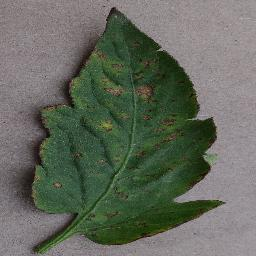
\includegraphics[scale=0.262]{./images/normal_3159}
	   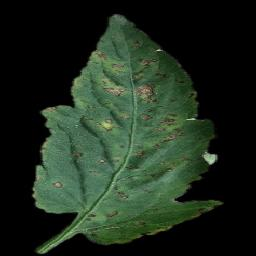
\includegraphics[scale=0.262]{./images/segmented_3159}
	   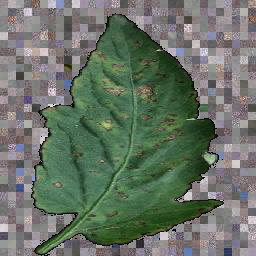
\includegraphics[scale=0.35]{./images/9_ROTATE_180_crop}
	   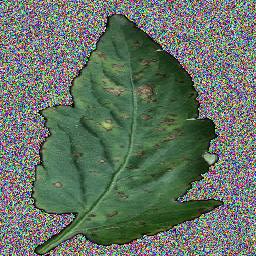
\includegraphics[scale=0.262]{./images/196_ROTATE_270}
	   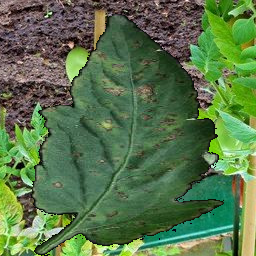
\includegraphics[scale=0.35]{./images/random_backgorund}
	   }
	\begin{center}
		\caption{Sampels of training images, from left to right: \textbf{Original PlantVillage dataset}, \textbf{Segmented PlantVillage dataset}, \textbf{Random background Crop dataset}, \textbf{Random Noise Backgorund} and \textbf{Random Background Image}}
		\label{fig:samples}
	\end{center}
	\vspace{-15pt}
\end{center}
\end{figure*}

\section{Experiments}
Our experiments are on two main task: Binary Classification, Multi-class Classification. In this section first we describe the dataset and the variations created to perform sensitivity analysis. Then we go trough the experiments setup were we describe how we have conducted the experiments to accomplish the two task and finally we show the results.

\subsection{Datasets}
We analyze 18158 images of tomato plant leaves, which are splitted in 10 classes, 9 diseases and 1 healthy. The scope is to predict the correct class of a leaf given its image. All the images are sized 256x256. 
\\\indent Given the original dataset we have conducted the training phase on different variations of the original dataset, we have worked on the background in order to find a way to overcome the limits highlined in \cite{} and confirmed by us.
In Figure \ref{fig:samples} we can see all the images the different versions of the dataset that we have tested and built.
\begin{itemize}
\item{\textbf{Original PlantVillage dataset} it consists of images of tomato leaves lain over a gray table.}
\item{\textbf{Segmented PlantVillage dataset} it consists of images of tomato leaves without the original background, this variation was used also in \cite{}. In our work we have re-segmented the images since in the available segmented dataset was not complete.}
\item{\textbf{Random Background Crop dataset} it consists of the leaf images coming from PlantVillage with a background composed of crops of background coming from the Original Plantvillage Dataset. We have tried this variation in order to exploit the dependence between original backgrounds and the class we found out in the experiment on the original dataset.}
\item{\textbf{Random Noise Backgorund} it consists of leaf images coming from PlantVillage with a background composed of random colored pixels. As before we tried this experiment to exploit the dependence between background and classes higlined in the original dataset.}
\item{\textbf{Random Background Image} it consists of leaf images coming form Plant Village with a background taken from a set of 4176 we built looking for tomato plantation images . The objective of this set was not only to exploit the backgorund influence on the classifier but also try to take the leaf in a situation similar to a realistic one, where the leaf image is taken directly in the plantation.}
\end{itemize}

\subsection{Experiments setup}
\subsubsection{Data Augmentation and Normalization}
As showed in Figure \ref{fig:1} after the Train-Test Split and Transformation Selection Phases our train set goes trough augmentation and normalization.
\\\indent We have performed data augmentation applying to the original sample two transformations from this pool:
Flip Top Bottom, 	Flip Left Right, Rotate 90\degree, Rotate 180\degree, Rotate 270\degree, Flip Top Bottom and Rotate 90\degree, Flip Top Bottom and Rotate 270\degree.
\\\indent After augmentation we have three samples for each original image (1 original image + 2 transformed images).
We have done this in order to train the networks with more data and strength the obtained model.
\\\indent Another key aspect of our setup is the normalization of the input images, the chosen normalization changes dramatically the validation accuracy. In our work we have explored the space of possible normalization considering these:
	\begin{itemize}
		\item{\textbf{Dataset Normalization} given the chosen variation of the dataset we have computed the mean and the standard deviation of the whole dataset.}
		\item{\textbf{Per-leaf Normalization} starting from the segmented dataset we have computed the mean and standard deviation of the non-black pixels.}
	\end{itemize}
\subsubsection{Binary Classification Setup}

\textbf{LeNet}
This network proposed in \cite{ref30} is one of the simplest deep model available. We have adapted it to perform our binary task. \\
\textbf{Weights Inizialization:}
for this network we started using training from scratch approach. The weights in the net are initialized using Xavier initialization \cite{ref31}. This helps training  since we start from a normally distribute set of weights and we avoid that certain weighs vanish trough epochs.
\\
\textbf{Activation Function:}
layers activation function is rectified linear unit (ReLU) since diminishes the likelihood of a gradient to vanish.
\\
\textbf{Loss Function:}
the chosen loss function for the binary classification is BCEWithLogitsLoss since it is designed for binary tasks and more stable compared to cross entropy.
\\
\textbf{Validation:}
for this task we have performed k-fold cross validation with k = 10 over the training set. This kind of validation was used to estimate the number of training epochs and the batch size to use.
\subsubsection{Multi-class Classification Setup}
\textbf{AlexNet}
for this task we have chosen a more complex model since we have tested LeNet over the ten class with results very far from the state of the art \cite{ref11}. In order to compare our results with \cite{ref11} we have chosen AlexNet.  \\
\textbf{Weights Inizialization:}
for this network we have tried both training from scratch approach and transfer learning. \\\indent The weights in the first case are initialized using Xavier initialization \cite{ref31}. This helps training  since we start from a normally distribute set of weights avoids that certain weighs vanish trough epochs.\\\indent In the transfer learning approach we have used the weights coming from the training on ImageNet \cite{imagenet}.
\\
\textbf{Activation Function:}
layers activation function is again rectified linear unit (ReLU).
\\
\textbf{Loss Function:}
in this case we have used Cross Entropy as loss function.
\\
\textbf{Validation:}
in the case of Multi-class Classification we opt to proceed with cross validation. We have chosen a different approach from binary classification. In fact k-fold cross validation applied on AlexNet requires a lot of computing time that is not justified in our dataset since there is small amount of variance in our pictures and consequently in each possible fold.
\\
\textbf{Optimizer:}
As optimizer we have choosen Adam \cite{ref32}. An important annotation should be done about this optimizer. In fact trough the training process we noticed that accuracy after a bunch of epochs drops. This was caused by the $\varepsilon$ coefficient, this coefficient used to avoid division by zero when the gradient is almost zero in parameters update.  By default is set to $1*10^{-8}$ and it causes large weights updates. So we set it to 0.1 to avoid this problem.

\begin{figure*}
\begin{center}
	\fbox{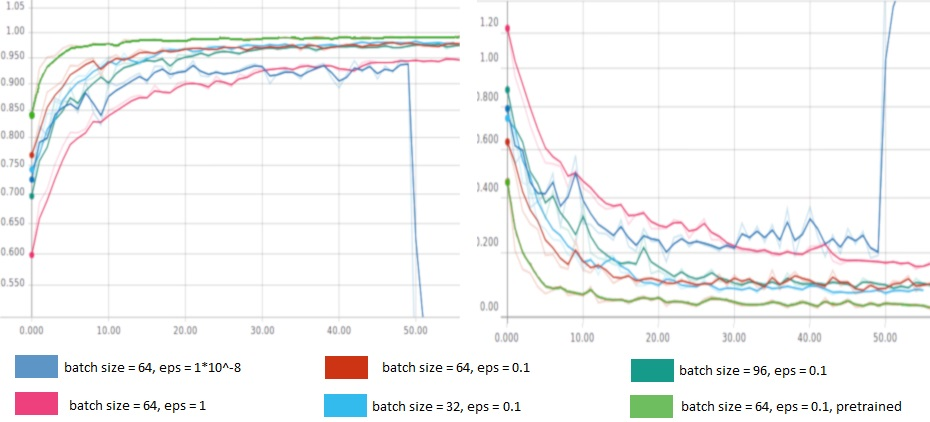
\includegraphics[scale=1.5]{./images/tensorboards}}
	\begin{center}
		\caption{Tensorboard graph of experiments, from left to right: \textbf{Validation Accurancy over epochs}, \textbf{Valdiation error over epochs}. }
		\label{fig:tensorboard}
	\end{center}
	\vspace{-15pt}
\end{center}
\end{figure*}

\subsection{Results and discussion}
\subsubsection{Binary Classification}
After a training phase using 10-fold cross validation, we select as best hyperparameters for our binary classification problem, the batch size equal to 32 and the total number of epochs equal to 15. With this configuration, after retraining the net on the global train set, we obtain the results on the test set shown in the table \ref{table:binary}. Beeing a very unbalanced dataset because of the number of healthy leaves with respect to the non healthy ones, we expected to have an healthy accurancy lower than non healthy. The result show that our assumptions was correct. In fact LeNet accurancy for healthy aren't good as for non healthy one. By the way the average performances of our net are good.
\begin{table}[H]
	\begin{center}
		\begin{tabular}{|l|c|}
			\hline
			\textbf{Measure} & \textbf{Results} \\ 
			\hline
			$Average Accuracy$ & $0.999184$ \\
			$Healthy Accuracy$ & $0.996678$ \\
			$Non Healthy Accuracy$ & $0.999407$ \\
			$Precision_M$ & $0.993377$ \\
			$Recall_M$ & $0.996678$ \\
			$F_1 score_M$ & $0.995025$ \\
			\hline
		\end{tabular}
	\end{center}
	\caption{Performance of binary classification.}
	\label{table:binary}
\end{table}
\subsubsection{Multi-class Classification}
As we did for binary classification, we try different run using different hyperparameters and we test our result on the validation set. As figure \ref{fig:tensorboard} shows, it's possible to understand that the best configuration it is given from Alexnet pretrained, with batch size equal to 64, eps equal to 0.1 for 57 epochs. The results obtained from this configuration are described in the first row of the table \ref{table:sensitivity}. AlexNet pretrained has a very good performance for all the classes and obtained also better result than the state of the art \cite{ref11}. We expected that classes with less samples, e.g. Tomato Mosaic Virus, would have been missclassified compared to classes with an higher number of samples, e.g. Tomato Yellow Leaf Curl. This do not happen in the reality, because our classifier missclassified only some samples that aren't related to the size of the class predicted.
\subsubsection{Sensitivity Analisys}
After having reached a good level of accuracy for our multi-class classification task, we move our attention to analise the robustness of our dataset by computing gradcam and occlusion methods to analise which parts of the leaf trigger the classifier. The table \ref{table:sensitivity} shows all the different approach we try. It's possible to see that the preformances of the results obtained are very far from the what we have done in the previous task. Sometimes also happens that some classes have never be predicted at all. Then we try in a different way, applying both normalization and backgrounds moving to something similar to what a predictor will see when it's applied on the field. Using per-leaf normalization and random background images we obtain the result shows in figure \ref{fig:conf_matrix}. It's also possibile to see in figure \ref{fig:gradcam} how the system is more robust to some background variation, activating only on the leaf surface.
\begin{table}
	\centering
	\small
	\begin{center}
		\begin{tabular}{|p{1.5cm}|p{1.5cm}|c|}
			\hline
			Train & Test & Performance\\ 
			\hline
			\multirow{4}*{Original}
			& Original & 
					\begin{tabular}{@{}c@{}}
					$Average Accuracy = 0.998560$ \\
					$Precision_M = 0.998339$ \\
					$Recall_M = 0.998173$ \\
					$F_1 score_M = 0.998254$ \\
					\end{tabular} \\
			\cline{2-3}
			& Segmented &
				\begin{tabular}{@{}c@{}}
				$Average Accuracy = 0.390169$ \\
				$Precision_M = NaN$ \\
				$Recall_M = 0.285877$ \\
				$F_1 score_M = Nan$ \\
				\end{tabular} \\  				
			\hline
			\multirow{4}*{Segmented}
			& Original & 
					\begin{tabular}{@{}c@{}}
					$Average Accuracy = 0.617933$ \\
					$Precision_M = 0.730197$ \\
					$Recall_M = 0.494125$ \\
					$F_1 score_M = 0.486940$ \\
					\end{tabular} \\
			\cline{2-3}
			& Segmented &
				\begin{tabular}{@{}c@{}}
				$Average Accuracy = 0.966511$ \\
				$Precision_M = 0.959517$ \\
				$Recall_M = 0.956894$ \\
				$F_1 score_M = 0.958019$ \\
				\end{tabular} \\  				
			\hline
			\multirow{4}*{Random Background Crop}
			& Original & 
					\begin{tabular}{@{}c@{}}
					$Average Accuracy = 0.769175$ \\
					$Precision_M = 0.794344$ \\
					$Recall_M = 0.673085$ \\
					$F_1 score_M = 0.671527$ \\
					\end{tabular} \\
			\cline{2-3}
			& Segmented &
				\begin{tabular}{@{}c@{}}
				$Average Accuracy = 0.848037$ \\
				$Precision_M = 0.885544$ \\
				$Recall_M = 0.737432$ \\
				$F_1 score_M = 0.739969$ \\
				\end{tabular} \\  				
			\hline
			\multirow{4}*{Random Noise Background}
			& Original & 
					\begin{tabular}{@{}c@{}}
					$Average Accuracy = 0.578862$ \\
					$Precision_M = 0.666754$ \\
					$Recall_M = 0.490099$ \\
					$F_1 score_M = 0.499304$ \\
					\end{tabular} \\
			\cline{2-3}
			& Segmented &
				\begin{tabular}{@{}c@{}}
				$Average Accuracy = 0.748469$ \\
				$Precision_M = 0.820938$ \\
				$Recall_M = 0.709873$ \\
				$F_1 score_M = 0.697417$ \\
				\end{tabular} \\  								
			\hline
		\end{tabular}
	\end{center}
	\caption{Performance of multi-class classification with difference training and test sets. We use a NaN value for the class that are never predicted to avoid division by zero in precision, recall and F1 score.}
	\label{table:sensitivity}
\end{table}
\begin{figure}[t]
	\begin{center}
		\fbox{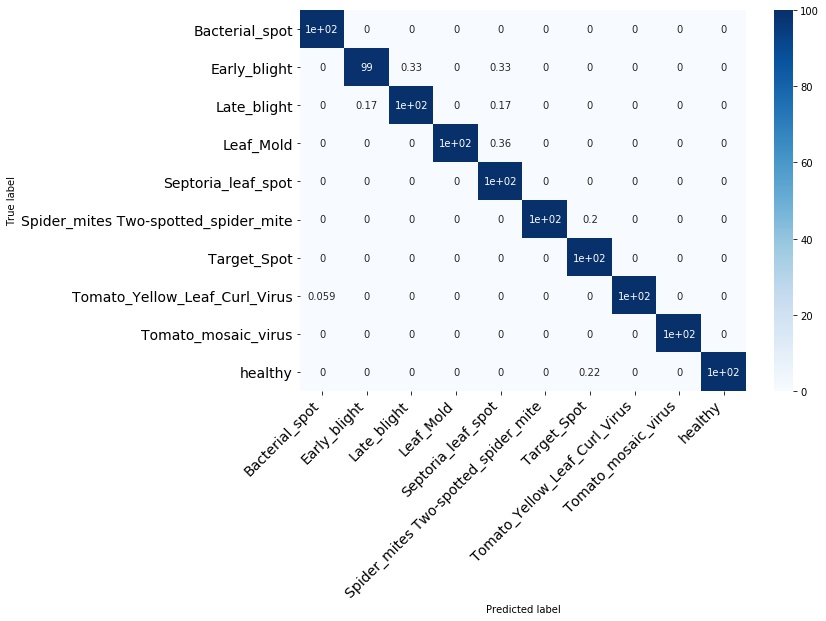
\includegraphics[scale=0.3]{./images/conf_matrix_norm}}
	\end{center}
	\caption{Confusion matrix of AlexNet pretrained in multi-class classification problem in percentage using per-leaf normalization and random background images.}
	\label{fig:conf_matrix}
	\label{fig:long}
	\label{fig:onecol}
\end{figure}
\begin{figure}[t]
	\begin{center}
		\fbox{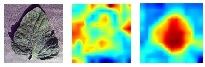
\includegraphics[scale=1]{./images/gradcam}}
	\end{center}
	\caption{From left to right: \textbf{Original image, class: Target Spot}, \textbf{GradCAM of AlexNet pretrained on Original dataset}, \textbf{GradCAM of AlexNet pretrained on random background images}. It is possible to see the difference on the activation of GradCAM, one is distributed both on the leaf and on the background, the other is locate only on the leaf disease.}
	\label{fig:gradcam}
	\label{fig:long}
	\label{fig:onecol}
\end{figure}

%-------------------------------------------------------------------------
\section{Conclusion}

%-------------------------------------------------------------------------
\section*{Acknowledgements}
aaa

%-------------------------------------------------------------------------
\appendix
\section{Supplementary Material}\begin{table}[H]
	\begin{center}
		\begin{tabular}{|l|c|}
			\hline
			\textbf{Measure} & \textbf{Formula} \\ 
			\hline
			$Average Accuracy$ & $\dfrac{\sum_{i=1}^{C} \frac{tp_i+tn_i}{tp_i+fn_i+fp_i+tn_i}}{C}$ \\
			$Precision_\mu$ & $\sum_{i=1}^{C} \frac{tp_i}{tp_i+fp_i}$ \\
			$Precision_M$ & $\dfrac{\sum_{\mu=1}^{C} Precision_\mu}{C}$ \\
			$Recall_\mu$ & $\sum_{i=1}^{C} \frac{tp_i}{tp_i+fn_i}$ \\
			$Recall_M$ & $\dfrac{\sum_{i=1}^{C} Recall_\mu}{C}$ \\
			$F_1 score_\mu$ & $\dfrac{2\times Precision_\mu \times Recall_\mu}{Precision_\mu+Recall_\mu}$ \\
			$F_1 score_M$ & $\dfrac{2\times Precision_M \times Recall_M}{Precision_M+Recall_M}$ \\
			\hline
		\end{tabular}
	\end{center}
	\caption{Measures of classification performance.}
	\label{table:1}
\end{table}
\begin{figure}[H]
	\begin{center}
		\fbox{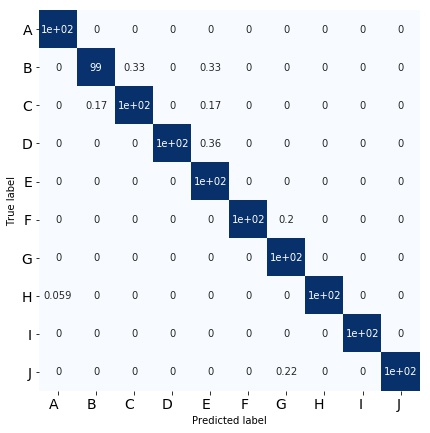
\includegraphics[scale=0.53]{./images/conf_matrix_norm-norm}}
	\end{center}
	\caption{\textit{Confusion matrix of AlexNet pretrained in multi-class classification problem in percentage using Orignal train against Original Test}}
	\label{fig:add1}
\end{figure}


\begin{figure}[H]
	\begin{center}
		\fbox{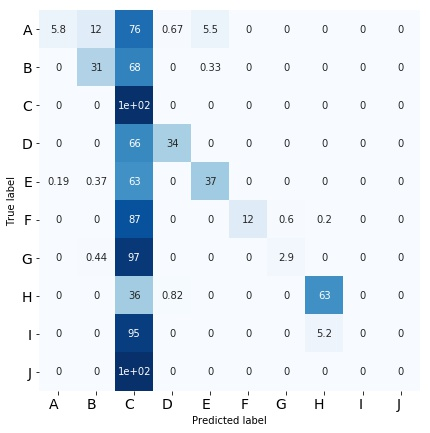
\includegraphics[scale=0.53]{./images/conf_matrix_norm_norm-seg}}
	\end{center}
	\caption{\textit{Confusion matrix of AlexNet pretrained in multi-class classification problem in percentage using Orignal train against Segmented Test}}
	\label{fig:add2}
\end{figure}
%-------------------------------------------------------------------------

{
	\small
	\bibliographystyle{ieee}
	\bibliography{bibliography}
}

\end{document}
